\documentclass[12pt,oneside,openany,a4paper,%..... Layout
               afrikaans, english,%.............. Global language selection
               ]{memoir}

 \usepackage[masters-t,%.......................... Master thesis
             goldenblock,%........................ A5 type block (or a5block or wide)
            ]{usthesis}%.......................... US thesis style with memoir

%
% PLEASE read the USthesis documentation for the class options
% and how to set line and paragraph spacing
%

%==== Language setup ================================================
 \usepackage[latin1]{inputenc}%................... Recognizes �, �, etc
 \usepackage{babel}%.............................. Language setup

%==== Math setup ====================================================
 \usepackage{amsmath}%............................ Advanced math (before fonts)
 %\usepackage{amssymb}%............................ AMS Symbol fonts

%==== Font setup (default is Computer Modern) =======================
 \usepackage[T1]{fontenc}%........................ Type 1 fonts
 %\usepackage{fourier}
 \usepackage{textcomp}%........................... Additional text character
 \usepackage{bm}%................................. Bold math symbols (after fonts)

%==== Ref's, Bib's and Nomencl ======================================
 \usepackage{usnomencl}%.......................... List of symbols (in usthesis pack)
 \usepackage{cite}
    \bibliographystyle{IEEEtran}
 % \usepackage{usbib}%.............................. Bibliography    (in usthesis pack)
 %    \bibliographystyle{usmeg-a}
 %    \renewcommand\bibfont{\small}

    %% For usmeg-a, the bib is a list of references. If you
    %% are using usmeg-n comment out the following lines
    % \addto{\captionsafrikaans}{\renewcommand{\bibname}{Lys van Verwysings}}
    % \addto{\captionsenglish}{\renewcommand{\bibname}{List of References}}

%==== Graphics and Color ============================================
\usepackage{graphicx}%........................... Graphicx loaded in usthesis
\usepackage{color}%.............................. Color setup
\usepackage{eso-pic}%............................ Shipout commands for watermark
    \newcommand*{\WaterMark}[2][0.15\paperwidth]{%
        \AddToShipoutPicture*{\AtTextCenter{%
                \parbox[c]{0pt}{\makebox[0pt][c]{%
                    \includegraphics[width=#1]{#2}}}}}}

%==== Local Defs ====================================================
\makeatletter

%
% Please insert user defined commands here
% and NOT in the document itself!
%

\makeatother

%==== TITLE PAGE ====================================================
\title{\bfseries
       \AorE{%-- Afrikaans ------------------------------------------
             Bitcoin betalingsraamwerk op 'n sosiale media platform\\[1ex]
             \normalfont\small\itshape
             (``Bitcoin payment framework on a social media platform'')
            }{%-- English -------------------------------------------
             Bitcoin payment framework on a social media platform
            }}

\author{W.\ Wessels}{Wessel Wessels}

\degree{\AorE{MIng (E\&E)}{MEng (E\&E)}}
       {\AorE{Magister in Ingenieurswese (Elektronies)}
             {Master of Engineering (Electronic)}}

\address{\AorE{%-- Afrikaans ----------------------------------------
        Departement Elektries en Elektroniese Ingenieurswese,\\
        Universiteit van Stellenbosch,\\
        Privaatsak X1, Matieland 7602, Suid Afrika.%
             }{%-- English ------------------------------------------
        Department of Electrical and Electronic Engineering,\\
        University of Stellenbosch,\\
        Private Bag X1, Matieland 7602, South Africa.
             }}

\faculty{\AorE{Fakulteit Ingenieurswese}%
              {Faculty of Engineering}}

\supervisor{Prof.\ G.\ van Rooyen}


\setdate{12}{2015}

%\SetSponsor{The financial assistance of the National Research Foundation (NRF)
%    towards this research is hereby acknowledged. Opinions expressed and
%    conclusions arrived at, are those of the author and are not necessarily to
%    be attributed to the NRF.}


%====================================================================
%     MAIN DOCUMENT
%====================================================================
\maxsecnumdepth{subsubsection}
\maxtocdepth{section}

\begin{document}

%==== Front matter ==================================================
 \frontmatter
 \WaterMark{UScrest-WM}
 \TitlePage

 \DeclarationDate{2015/12/10}
 \DeclarationPage

 \begin{abstract}[english]%===================================================
English abstract to be written
\end{abstract}


\begin{abstract}[afrikaans]%=================================================
Afrikaanse uittreksel wat nog geskryf moet word
\end{abstract}


\chapter{Acknowledgements}%==================================================

I would like to express my sincere gratitude to the following people
and organisations ...


\chapter{Dedications}%=======================================================
 \vfill
 \begin{Afr}
 \begin{center}\itshape
    Hierdie tesis word opgedra aan ...
 \end{center}
 \end{Afr}
 \vfill
 \clearpage

%============================================================================
\endinput


 \tableofcontents
 \clearpage

 \setcounter{lofdepth}{2}
 \listoffigures
 \clearpage

 \listoftables
 \clearpage

 \chapter{Nomenclature}
 No nomenclature yet.
% \begin{Nomencl}
%  \NomGroup{Constants}%-----------------------------------------------
%    \item[$\mathrm{g} = $] $\mathrm{9.81\,m/s^2}$

%  \NomGroup{Variables}%-----------------------------------------------
%    \item[$\mathit{Re}_\mathrm{\,D}$]
%                       \UnitLine{Reynolds number (diameter)}{~}
%    \item[$x$]         \UnitLine{Coordinate                }{m}
%    \item[$\ddot{x}$]  \UnitLine{Acceleration              }{m/s^2}\\
%    \item[$\theta$]    \UnitLine{Rotation angle            }{rad}
%    \item[$\tau$]      \UnitLine{Moment                    }{N{\cdot}m}

%  \NomGroup{Vectors and Tensors}%-------------------------------------
%    \item[$\overrightarrow{\bm{v}}$] Physical vector, see equation ...

%  \NomGroup{Subscripts}%----------------------------------------------
%    \item[$\mathrm{a}$] Adiabatic
%    \item[$a$]          Coordinate
% \end{Nomencl}



\endinput


%==== Main document =================================================
\mainmatter
   \setsecnumdepth{subsubsection}
%   \numberwithin{equation}{section}
%   \numberwithin{figure}{chapter}
%   \numberwithin{table}{chapter}

%!TEX root = ../USthesis_Masters.tex
\chapter{Introduction}
\label{chp:Intro}

Bitcoin \cite{Nakamoto2008} is a peer-to-peer decentralised digital payment mechanism that was introduced in a paper published by a person or group called Satoshi Nakamoto in 2008. Bitcoin aims to be an alternative to traditional centralised online payment mechanisms like credit cards and PayPal \cite{PayPal2015}. 

We focus on testing the viability of Bitcoin as payment mechanism on social media platforms, specifically on a mobile platfom. 

To test the viability, we will design a Bitcoin payment framework that allows developers to incorporate Bitcoin payments in their applications without having to understand the low-level details of Bitcoin and without running any Bitcoin software.

We will also design and build a Bitcoin wallet application that will run on the social media platform to make payments directly from the application. 


%%%%%%%%%%%%%%%%%%%%%%%%%%%%%%%%%%%%%%%%%%%%%%%%%%%%%%%%%%%%%%%%%%%%%%%
\section{Background}

Making payments on a mobile social media platform has been done in several different ways in the past. One of the biggest challenges to overcome is that many users don't have a credit card. For many social media platforms, this is especially true since the target audience of the platform is teenagers. 

With Apple's in-app purchases \cite{apple}, credit card details have to be loaded in only once. A parent can thus load a credit card for a child and let the child use it, but this can lead to problems of unregulated spending.

Another common method of payment is using mobile airtime as payment. Airtime is very easy to use, but the cost to the merchant is very high.

The last payment method we look at is a voucher based system, like Apple's Gift Cards. Vouchers are very similar to airtime as payment, but the voucher credit can only be used on the specific platform. Vouchers, like airtime, can be purchased at supermarkets. However, since the voucher is issued by the company with only the supermarket as middle-man, it follows that the loss that the company makes on overhead is less than with airtime.

We would like to test the viability of Bitcoin as an alternative to these methods of payment, especially to take advantage of Bitcoin's low transaction fees.

Bitcoin transactions can be processed without any transaction fee, but a small fee may be required for transactions that uses a lot of unspent outputs and thus causes a larger transaction. A large transaction in Bitcoin refers to the amount of bytes that the transaction uses and not the value of the Bitcoin. A small fee can also be added to speed up the processing time of the transaction. There are criticisms that say that the low price of transaction fees are unsustainable and will likely increase in the future \cite{Ka2014}.



\section{Related Work}

To compare Bitcoin as a payment method on a social media platform, we must look at existing payment methods and their advantages and disadvantages. 

\subsection{Credit and Debit Cards}

\begin{table}
	\begin{center}
		\begin{tabular}	{ | c | c | c |}
		\hline
		Credit Card & Debit Card & PayPal \\ \hline
		48\% & 30\% & 12\% \\ \hline
	 
	   % \label{fig:htaccess_file}
		\end{tabular}
		\caption{Table of preferred online method of payment \cite{tsys}} 
		\label{tbl:preferred_payment}
	\end{center}
\end{table}

According to a study done in 2014 \cite{tsys}, 48\% of people prefer to make online payments with credit cards and 30\% prefer debit cards. It is clear from these statistics that these traditional payment methods are still very prevalent. 

\subsubsection{Advantages}

Credit card payments are easy to make and are processed quickly. The cost of transactions are very difficult to determine, as they differ from bank to bank, where you buy and the user's specific credit card package. However, credit card payments can be very cheap, since they usually have a small fixed and percentage fee per payment that is paid by the merchant. Since credit cards are backed by a trusted third-party, they are able to provide mediation when desputes arrive. They can also provide insurance against fraud. 

\subsubsection{Disadvantages}

According to a survey done in 2014, 75\% of adult South Africans are banked \cite{finmark}. A quarter of the adults do not have bank accounts, making it almost impossible for them to purchase anything online. Furthermore, there are prerequisites to getting a credit card, like minimum income. Credit cards also usually have a fixed monthly fee.

Using a credit card is not anonymous, since the user has to enter the card number for each payment. Every payment made by the user is thus traceable by the credit card company. This may be a concern to certain people.

Even though credit cards have very small transaction fees, they still have a small fixed fee. This is an issue when payments are very small. For example, the company PayFast \cite{PayFast} charges a fixed R2 and 3.9\% of the payment as a fee. Thus, when a user wants to make a R5 payment, the merchant will only receive $R5 - R2 - R5 \times 3.9\% = R2.81$.


\subsection{Airtime Payment}

A popular mobile messaging application, Mxit, uses airtime payments with its Mxit Moola \cite{Mxit} virtual currency. They use a system where a user sends an SMS to a specific number to make a payment. For example with Mxit Moola, a user will send an SMS costing R3 of their airtime and receive 300 Moola. This is very convenient for the user, however it is not very profitable for the company.

\begin{table}
	\begin{center}
		\begin{tabular}	{ | c | c | c | c | c |}
		\hline
		SMS Cost & Vodacom & MTN & Cell C & 8ta \\ \hline
		R1.00 &	R0.07 &	R0.06 &	R0.09 &	R0.04 \\ \hline 
		R1.50 &	R0.44 &	R0.31 &	R0.37 &	R0.27 \\ \hline
		R2.00 &	R0.81 &	R0.56 &	R0.66 &	R0.52 \\ \hline
		R3.00 &	R1.55 &	R1.08 &	R1.24 &	R0.99 \\ \hline
		R5.00 &	R3.03 &	R2.11 &	R2.40 &	R2.06 \\ \hline
		R7.50 &	R4.88 &	R3.39 &	R3.84 &	R3.31 \\ \hline
		R10.00 & R6.73 & R5.10 & R5.29 & R4.57 \\ \hline
		R15.00 & R10.43 & R7.24 & R8.18 & R7.07 \\ \hline
		R20.00 & R14.13 & R9.81 & R11.14 & R9.58 \\ \hline
		R25.00 & R17.83 & R10.91 & R13.96 & R12.10 \\ \hline
		R30.00 & R21.53 & R14.40 &	R16.85 & R14.60 \\ \hline
	 
	   % \label{fig:htaccess_file}
		\end{tabular}
		\caption{Table of SMS payment payouts from bulksms.com \cite{bulksms.com}} 
		\label{tbl:sms_prices}
	\end{center}
\end{table}

\begin{figure}
  \centering
    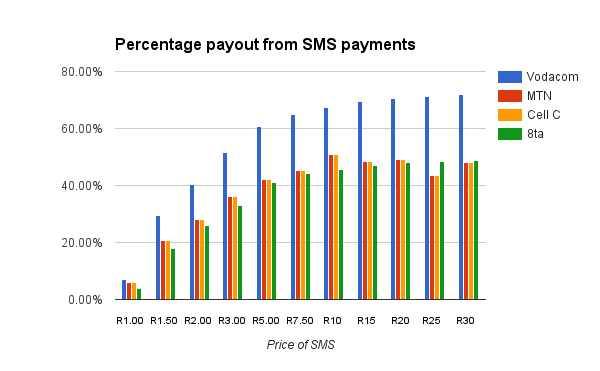
\includegraphics[width=0.9\textwidth]{figs/sms_percentage.png}
   \caption{Graph showing payout percentages for SMS payments} 
   \label{fig:sms_percentage}
\end{figure}

From table \ref{tbl:sms_prices} and figure \ref{fig:sms_percentage} we can see that the company itself gets a very small percentage of the payment. This is especially true for payments less than R5, where the average payout percentage is less than 50\%. Even the highest SMS value at the network with the highest payout only has a payout of 71.77\%.

\subsubsection{Advantages of Airtime}

The airtime model works very well, because it allows teenagers to use it with their existing airtime quotas without requiring their parents credit card details. Airtime is also very easily accessible, since it can be bought with cash at most supermarkets among other methods. 

\subsubsection{Disdvantages of Airtime}

Airtime as payment only has one big disadvantage - the very high transaction fee paid by the merchant. 


\subsection{Vouchers}

Vouchers are very similar to airtime in regards to accessability. A physical voucher can usually be bought at a supermarket, where a code is sold to the user. This code is then entered by the user on the service provided by the company that provides the voucher, where the user will then receive the amount of the voucher as credit. For mobile purchases, Apple's Gift Cards are a very good example of vouchers in practice. The gift cards can be used in all the same Apple-related online stores that credit cards are used. This allows users to effectively buy online virtual goods using cash.

\subsubsection{Advantages of Vouchers}

Vouchers are easily accessible and are purchasable using cash. They are comparable to the airtime payment model, but they provide more controll to the merchant. Vouchers also enable users to budget their spending, something that is ideal for teenagers and children.

\subsubsection{Disadvantages of Vouchers}

Vouchers can only be used at the online merchant that they are bought for. Thus, if a person wants to pay at different online merchants, they will need to buy a voucher for each of the merchants. 

Since a voucher is a physical item, it has to be manufactured and distributed across the world. This adds to the overhead cost, and it is possible for vouchers to be sold out in certain places.

\section{Objectives}

Our objective is to test the viability of Bitcoin as a payment mechanism on a social media platform. The platform we chose is a text-messaging social media application called WeChat.

We want to test how Bitcoin compares to alternative payment mechanisms on the following criteria:

\begin{itemize}
	\item{Transaction fees}
	\item{Ease of use}
	\item{Versatility}
\end{itemize}
% In granular or particle flow simulations with Discrete Element Method (DEM),
% the mechanical behavior of a system of particles are simulated. The basic
% building blocks of DEM are finite sized particles and walls. It is generally
% classified into two basically different approaches.

% The first is the ``hard sphere'', event-driven method
% \citep[e.g.][]{Luding-1994, Luding-2004}, where particles are assumed to be
% perfectly rigid and they follow an undisturbed motion until a collision
% occurs. Due to the rigidity of the interaction, the collisions occur
% instantaneously with accompanying momentum transfer. It is mainly used for
% collisional, dissipative granular gases.

% The second is the so-called ``soft particle'' molecular dynamics pioneered by
% \citet{Cundall-1979}, where the particles are allowed to overlap or penetrate
% each other. Constrains on the physical space that a particle can occupy at a
% specific time is included with contact or penalty forces related to the
% amount of overlap and contact velocity between particles or between particles
% and walls. The motion of the system is modelled by the integration of
% Newton-Euler equations for motion of every individual particle.

%!TEX root = ../USthesis_Masters.tex

\chapter{Literature Study}
\label{chp:literature_study}



%%%%%%%%%%%%%%%%%%%%%%%%%%%%%%%%%%%%%%%%%%%%%%%%%%%%%%%%%%%%%%%%%%%%%%%
\section{Bitcoin}

Bitcoin is a highly technical protocol that was introduced in 2008. For this project we will look at the relevant practical characteristics of the Bitcoin network as it is implemented in the real world.

The code that is responsible for the Bitcoin network is open source and is maintained by a core team of developers. Since the code is open source, anyone can verify the code to ensure it is not malicious. The Bitcoin network also chooses what code to run, so consensus must be reached between the Bitcoin network and the software.

Bitcoin is decentralised, which means no central authority controls the network. Rather, Bitcoin is run by independant nodes that work together.

Bitcoin uses cryptography to remove trust from a central authority.

\subsection{A Bitcoin Address}

A Bitcoin address has two parts, a private key and a public key. The private key is an unsigned 256 bit integer that is usually randomly generated, but can also be chosen by the user. This private key should be kept secret, as anyone with the key can spend any Bitcoin that belongs to it.

The public key is generated from the private key using a combination of Elliptic Curve Digital Signature Algorithms and several hashing functions. A private key can't be determined by knowing the public key, and thus it is safe for the public key to be known by anyone.

An analogy of a postal box can be used to explain a Bitcoin address. The public key is like a post box. Anyone can deposit something into the box without having access to the key of the box. They only need to know the box number to make the deposit. To retrieve or spend whatever is in the box, we need the key. Thus, the private key is like the key to the post box. Only the person with the key can open the box. One important difference to a normal postal box is that the postal box is completely transparent, meaning anyone can see exactly what is in the box.

\subsection{How Bitcoins Are Stored}
\label{sbs:bitcoin_stored}

Bitcoin is ``stored'' using a public ledger called the blockchain. Effectively, every single successful Bitcoin transaction is stored in this public ledger, and every user that runs a full Bitcoin node has an identical copy of the blockchain. The authenticity of the blockchain is managed by using consensus on the network and using hashing alogrithms. Bitcoin transactions are bundled into blocks, and the entire block is hashed. This block is hashed with the hash of the previous block as input, and so forth in the chain until the first block is reached. Thus, every block's hash is the hash of the entire chain behind it. This means that nothing can be changed in the chain, since it will change the entire hash after the change.

Since the entire ledger of Bitcoin transactions are available, it is possible to calculate the balance of any address at any given time. Since there are so many copies of the blockchain, only the Bitcoin private key is required to be stored. Even though the public key is calculated from the private key, a server usually stores the public key as well since it will be inefficient to calculate it everytime we a lookup is needed. The fact that we only need to store these two values in order to have access to the Bitcoin is the most relevant part of how Bitcoin works for our purposes. It allows a developer to simply store these simple two values securely, without having to keep track of ledgers locally.

\subsection{How a Bitcoin Transaction Works}

Since the blockchain is a public ledger of all transactions, it is a crucial part of making a new transaction. Every transaction has inputs and outputs. When looking at an address at a specific point in time, we can determine which of the outputs of its transactions are not spent yet. They are called unspent outputs. These outputs can be cryptographically verified to belong to a specific address. These outputs can be used as inputs in a new transaction. The transaction then specifies new outputs to send Bitcoin to. To receive ``change'' in a Bitcoin transaction, the change amount must be specified to the address that the payer chose. The change address can be a new address owned buy the payer, or the same address that the payment came from.

The difference between the inputs and outputs of a transaction is the transaction fee that is claimed by users that verify transactions. 

\subsection{Bitcoin Mining}

Bitcoin Mining is the process of bundling transactions together to form a block. As mentioned in \ref{sbs:bitcoin_stored}, every block has a hash that is in effect the hash of the entire chain. For a block to be valid, this hash has to satisfy the condition of leading with a certain amount of zeroes. This concept is arbitrary. Its only purpose is to be difficult to do, so that a lot of work is required to do so. The only way of doing this is using a brute force method. Thus, more computation power increases the odds of finding a block that satisfies the zeroes criteria.

The amount of zeroes required is called the ``difficulty'', since more zeroes make it more difficult to find a valid block. The amount of zeroes required is dynamically updated by the Bitcoin network to ensure that the average time for finding such a block is 10 minutes.

When a transaction is mined into a block, we say it has 1 confirmation. The longer the chain becomes after this block, the more confirmations it has and we can with higher trust say that the transaction is final. For example, a transaction with only one confirmation can still be rejected if a successful double-spend attack is done. With more confirmations, the probability of doing a double-spend attack lowers exponentially \cite{Nakamoto2008}. With very small payments, we do not require many confirmations to accept a payment. It is worth the risk of accepting a payment with 0 confirmations, since it is not worth the effort to try and do a double-spend on such a small transaction.




%!TEX root = ../USthesis_Masters.tex
\chapter{System Design}
\label{chp:System Design}


%%%%%%%%%%%%%%%%%%%%%%%%%%%%%%%%%%%%%%%%%%%%%%%%%%%%%%%%%%%%%%%%%%%%%%%
\section{Framework}

In this project we test the viability of a payment framework on a mobile social media platform. The framework will consist of several independant but connected pieces:

\begin{itemize}
	\item REST API for payments
	\item Wallet Application
	\item Bitcoin Interface
	\item Use-case Application
\end{itemize}

A summary of what is required from the system can be seen in figure \ref{fig:summary_framework}.

\begin{figure}
  \centering
    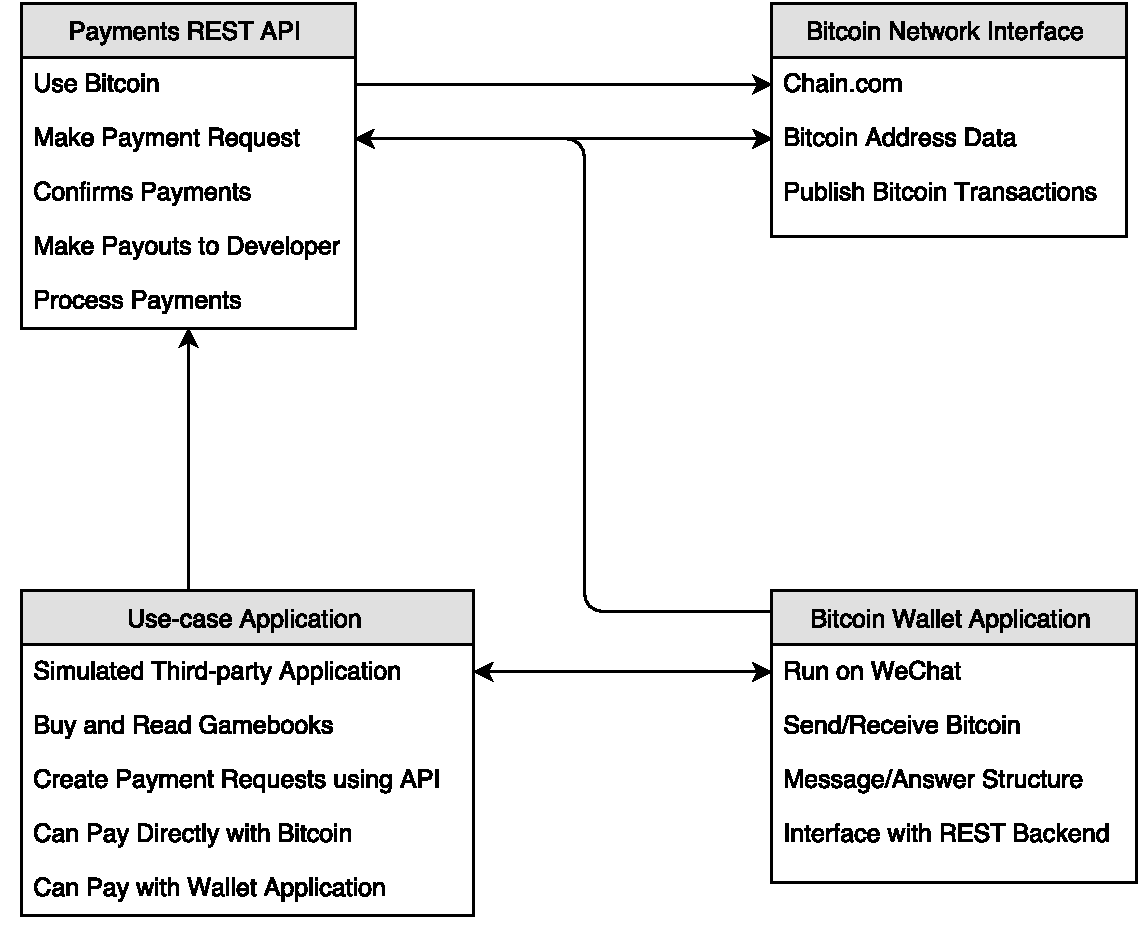
\includegraphics[width=0.7\textwidth]{figs/Summary.pdf}
   \caption{Summary of Framework} 
   \label{fig:summary_framework}
\end{figure}

\subsection{REST API for payment management}

A REST (Representational State Transfer) API \cite{Oracle.com} was chosen for the main interface for developers to use Bitcoin without running a Bitcoin node or having experience with Bitcoin. REST was chosen because it is a commonly used architecture, it is easy to use and understand and it does not constrain the user's choice of programming langauge or environment. 

The purpose of the REST API is to let developers make payment requests and check if a payment has been made, without dealing with the low-level Bitcoin transactions directly. Thus, our system should generate a new Bitcoin address on request. 

% We also require the developer to check wether a payment has been successfully made.
Our requirements from the REST API are:

\begin{itemize}
	\item New Bitcoin address for each payment
	\item Verify payment
	\item Check total balance of developer
	\item Witdraw available Bitcoin of developer
\end{itemize}

\subsubsection{The concept of the Bitcoin payment}

This is a high-level explanation of how to receive verifyable payments with Bitcoin. With Bitcoin, unlike a traditional bank account, you don't have a single ``account'' where people can make payments to and you can verify that the payment came from them. With Bitcoin it is trivially easy to make a new Bitcoin address, and it can be generated without being connected to the Internet or the Bitcoin network.

Since the entire Bitcoin blockchain is public, a single address is not sufficient to receive multiple payments. With a single address, it is not easy to verify that a spesific person has made a payment, since there may be several payments of the same amount happening in short succession.

The sollution to the problem is generating a new address for every payment, and requesting that the user make the payment to that address. Since the newly generated address is not yet present on the blockchain, when a payment to that address of the requested amount occurs, we can be certain that the person in question made the payment. When the payment is complete, the Bitcoin in that address can be transferred to a central address, and the original address can be discarded.

From our requirements for the REST API, we clearly require (at least) the following methods:

\begin{itemize}
	\item A ``payment'' method
	\item A ``balance'' method
	\item A ``payout'' method
\end{itemize}

\subsubsection{The /payment method}
\label{sct:payment}

The /payment method is the core of the REST API. It is used to make a payment request with a specified amount of Bitcoin and a description of the transaction. The /payment method returns a Bitcoin public address and a payment ID. 

The user can then pay to the Bitcoin address using any standard Bitcoin payment method, or can pay directly from the Bitcoin wallet that will run on WeChat and will be connected to the payment infrastructure.

\subsubsection{/payment/\{PUBLIC\_ADDRESS\} and /payment/\{ID\}}

These two methods are conceptually the same, but they take in two different arguments. The one takes the Bitcoin address to be queried, and the other takes the payment ID. The method returns all the data about the transaction, including the status of the transaction. 

The main purpose of this method is to verify that a transaction has been completed by the user. It can also be used to give the payment details to to user again.

\subsubsection{/balance}

The /balance method gives the developer the balance of all the available Bitcoin from all the received transactions. The method also returns a flag that says if there is enough Bitcoin to make a payout.

\subsubsection{/payout}

The /payout method is used by the developer to transfer all of the available Bitcoin to a specified Bitcoin address.

\subsection{Wallet Application}

The Wallet Application is a Bitcoin wallet implemented on the WeChat platform. The WeChat platform uses a simple message-answer structure. A user sends a message in the Wallet Application. The message is then sent to WeChat that sends it to a third party server controlled by the developer. The server then sends a reply to WeChat that is then forwarded to the user. 

In this manner, a fully functional Bitcoin wallet is realised. The third party server stores the private keys and processes the Bitcoin transactions on commands from the user.

The advantage of using the WeChat platform is the security built in to the platform, as well as an existing userbase. 

The Wallet Application will be directly connected to the back-end of the REST API. Thus, payment requests will be referable directly from the Wallet Application without needing to reference the Bitcoin Address. It will be able to reference the request using the payment ID mentioned in \ref{sct:payment}

\subsection{Bitcoin Interface}
\label{sct:bitcoin_interface}

To connect to the Bitcoin peer-to-peer network, a Bitcoin client is needed. The standard way of doing this is running the Bitcoin open source software on a server. This is very network and processor intensive. For development and testing, it will be quite expensive to run the Bitcoin software. Thus, an alternative is required for interfacing with the Bitcoin network. Fortunately, there are services that provide access to most of the Bitcoin operations using their API's. 

We require the following from such a service:

\begin{itemize}
	\item Get the balance from an address,
	\item Get unspent outputs from an address,
	\item Post a signed Bitcoin transaction to the network,
	\item It must be able to use the Testnet
\end{itemize}

The details of the chosen service is covered in chapter \ref{chp:Detail Design}.
% After considering several options, a service called chain.com was chosen. Chain.com is a free service that satisfies all the requirements. It is perfect to use this service as a proof of concept, but in practice one would rather run a full Bitcoin node to minimize reliance on third-party services.

\subsection{Use-case Application}

To use the payment framework, a Gamebook application is created to read Choose Your Own Adventure style books on the WeChat platform. User-created books can be sold by using the Bitcoin payment framework and the author can potentially earn Bitcoin.

For each sale, the Gamebook application creates a payment request using the REST API. The user can then pay using the Wallet Application or any Bitcoin payment mechanism. The Gamebook application can the query the API to confirm that the payment is received. 
%!TEX root = ../USthesis_Masters.tex
\chapter{Detail Design}
\label{chp:Detail Design}


%%%%%%%%%%%%%%%%%%%%%%%%%%%%%%%%%%%%%%%%%%%%%%%%%%%%%%%%%%%%%%%%%%%%%%%
\section{Back-end}

To implement the payment framework, we need a back-end server and a back-end web framework. 

\subsection{Back-end Server}

We chose an Amazon Elastic Cloud Computing (EC2) instance for the back-end server. EC2 gives us access to a virtual machine (VM) where we can run our own software, including a publicly accessible website. The micro instance is deployed in Singapore in the Asia Pacific region. The reason for this is to have the server as close as possible to the WeChat servers in China, since our servers must connect to WeChat's servers.

\subsection{Back-end Web Framework}

We decided to use XAMPP (Apache, MySQL, PHP and Perl) for the back-end development environment. XAMPP is a full stack development environment. It includes an HTTP server (Apache), a database server (MySQL) and a scripting language (PHP). XAMPP is free and easy to deploy, and is also used because the author is familiar with it.

\section{Social Media Platform}

We chose WeChat for our social media platform. WeChat works on most smartphones, already has a userbase and it has a third-party API with a development sandbox feature. 

On WeChat, a third-party application is known as an ``Official Account''. We registered for a sandbox Official Account that only allows 20 users and is not searchable on WeChat.

WeChat acts as an intermediary between the user and our server as seen in figure \ref{fig:wechat_interaction}. 

\begin{figure}
  \centering
    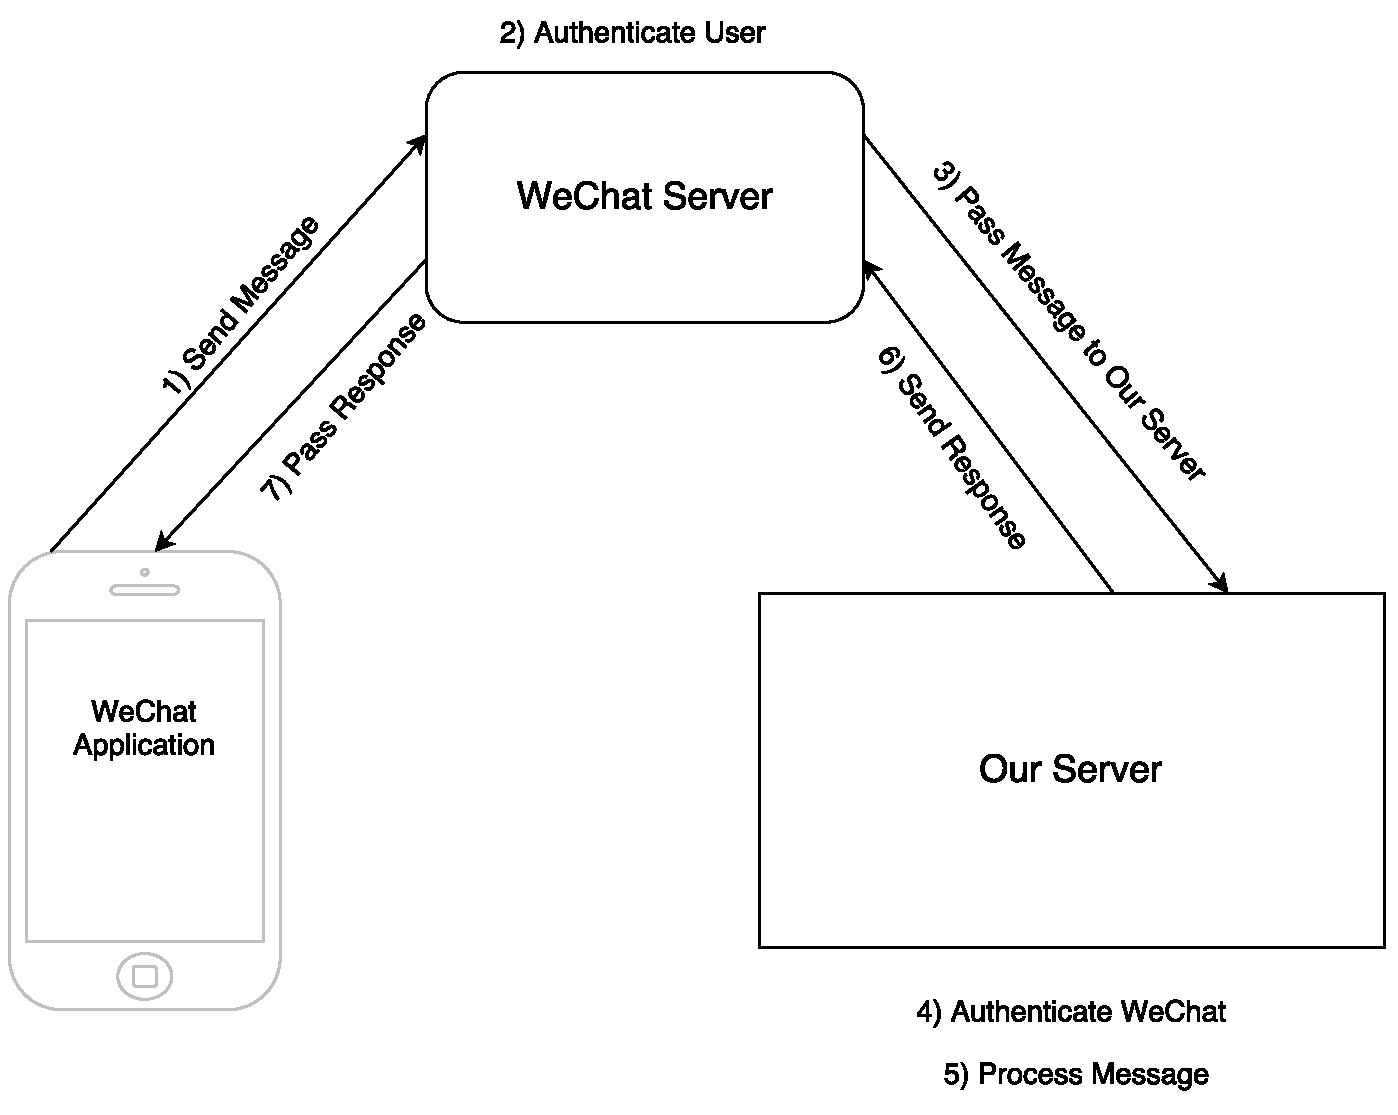
\includegraphics[width=0.7\textwidth]{figs/Wechat_interaction.pdf}
   \caption{Interaction with WeChat} 
   \label{fig:wechat_interaction}
\end{figure}

WeChat uses a shared token hashing scheme to authenticate itself on our service. We provide 
%!TEX root = ../USthesis_Masters.tex

\chapter{Tests}
\label{chp:Tests}


%%%%%%%%%%%%%%%%%%%%%%%%%%%%%%%%%%%%%%%%%%%%%%%%%%%%%%%%%%%%%%%%%%%%%%%
\section{Quantitative}

This project is an implementation of a platform on top of an existing social media platform WeChat. We do not have access to the back-end systems of WeChat. This makes it hard to do many of the quantitative tests required for the application itself. They will require qualitative tests. The REST API however, can be tested thoroughly using unit tests. 

\subsection{REST API unit tests}

There are tools and frameworks available for testing REST API's. Just like when making the REST API, we decided to rather write the unit tests ourselves without using a framework in order to get a better understanding of how unit tests work.

Thus, we wrote the entire REST API unit tests in a PHP script that calls all our REST endpoints with inputs that we know what the outputs should be. Each test should also confirm that the correct HTTP status code, as shown in table \ref{tbl:http_status_codes},  is returned. In total, there are 39 different tests that excecute. 

\begin{table}
	\begin{center}
		\begin{tabular}	{ | c | c | p{5cm}|}
		\hline
		Status Code & Text & Description \\ \hline
		200 & OK & Request succeeded \\ \hline
		400 & Bad Request & Request not understood due to malformed syntax \\ \hline
		401 & Unauthorized & The request requires user authentication \\ \hline
		404 & Not Found & Request does not exist \\ \hline
		
	   % \label{fig:htaccess_file}
		\end{tabular}
		\caption{Table of selected HTTP status codes} 
		\label{tbl:http_status_codes}
	\end{center}
\end{table}



\subsubsection{Testing Authentication}
In order to test the authentication of the developer with our REST API, we wrote a simple endpoint called /test that returns an HTTP status code ``200 OK'' if the authentication was successful and the corresponding status code if it is unsuccessful.



The following are the tests that should not authenticate:

\begin{itemize}
	\item Duplicate Request
	\item Missing api\_key
	\item Invalid api\_key
	\item Missing nonce
	\item Missing timestamp
	\item Missing signature
	\item Invalid signature
\end{itemize}

Since all of these tests fail to authenticate, they should all return an HTTP status code ``401 Unauthorized''.

All further tests assume that the authentication happens successfully.

\subsubsection{Testing /payment}

To test the /payment endpoint, we make a payment request with an amount and a description. For the result, we expect a valid Bitcoin address with the same amount and description that we provided. We uses a function in bitcoin-lib-php library to validate the Bitcoin address. 

The following are tests that should fail:

\begin{itemize}
	\item Wrong Method (GET instead of POST)
	\item amount\_sat smaller or equal to 0
	\item amount\_sat not an integer
	\item Missing description
	\item Description too long
\end{itemize}

These tests should all return an HTTP status code ``400 Bad Request''.

\subsubsection{Testing /payment/\{TRANSACTION\_ID\}}

To test this method, we need to call it with a valid transaction ID that corresponds to the api\_key that created the transaction. If the ID does not correspond with the api\_key, the test should return an HTTP status code ``401 Unauthorized''.

\subsubsection{Testing /payment/\{PUBLIC\_ADDRESS\}}

Testing this method is very similiar to the /payment/\{TRANSACTION\_ID\}. The public address must correspond with the api\_key that created the transaction. 

The following tests should fail:

\begin{itemize}
	\item Wrong Public Address (401 Unauthorized)
	\item Invalid Public Address (400 Bad Request)
\end{itemize}

\subsubsection{Testing /balance}

This method only has no arguments. Thus, if the authentication succeeds, it should return an HTTP status code ``200 OK'' and the balance.

\subsubsection{Testing /payout}

This method will always return an HTTP status code ``200 OK'' with the result in the JSON response. 

The following tests should fail:

\begin{itemize}
	\item No Address Given
	\item Invalid Address
\end{itemize}

\subsubsection{Testing Invalid API Method}

All these tests should return an HTTP status code ``404 Not Found'':

\begin{itemize}
	\item No Method Given
	\item Testing ``/''
	\item Testing /asdfasdf
	\item Testing /asdfasdf/asdfasdf
	\item Testing /balance/asdfasdf
	\item Testing /payment/asdfasdf
\end{itemize}	

	
\section{Qualitative}

Since we are implementing a system that is used by people, a large part of our testing is qualitative.

We wrote a guide that goes step-by-step through the processes of using the systems that we have built.

The user is asked to add the Wallet Application inside WeChat and then load some Testnet Bitcoin to their wallet from a website that gives free Testnet away. This is to let them understand the concept of loading Bitcoin to their Wallet. They are then asked to write a small Gamebook on the Gamebook Author page. They only need to write three pages: one start page that links to two pages.

After they finished the Gamebook, they are asked to add the Gamebooks Application inside WeChat. They should then navigate in the Gamebooks Application to the small story they just wrote and buy it. When they select it, they will receive a payment ID that they must enter in the Wallet Application and confirm the payment. They should then be able to read the story they just wrote and bought.

To get feedback, we wrote a Google Form to make a questionnaire. The advantage of using a Google Form is that it directly outputs the answers of the users in a single spreadsheet.

The main things we wanted to learn from the feedback was how easy the users where able to use the payment mechanism and how viable it is compared to traditional payment mechanisms.

\subsection{Feedback}

90\% of users used an iPhone when testing. The reason for this being so high is that a phone was offered for them to use in case they didn't have WeChat installed on their own phone. 10\% of users had an Android device, and the test was successful.

60\% of users never used WeChat before this test, and the other 40\% have used it before, but they no longer use it.

20\% of users are familiar with Bitcoin, with 70\% saying they have heard about it and 10\% saying they have never heard about it. 

90\% of users where able to add the Wallet and Gamebooks Applications within WeChat on the first try, with 10\% being able to add it with some trouble.

60\% of users said that the Wallet Application is easier to use than traditional payment mechanisms, with 20\% saying they are the same an 10\% said that traditional payment mechanisms are easier.

50\% of users said that the Wallet Application is faster than traditional payment mechanisms, with 30\% of users saying they are the same and 20\% saying that traditional mechanisms are faster.

We asked users what payment mechanism they would prefer to use assuming that Bitcoin is more easily accessible. 50\% of users said they would prefer Paypal, with 40\% of users saying they prefer the Wallet Application and 10\% saying they prefer a debit card.

The users were asked to rate the Wallet Application overall out of 10. The average rating is 7.8, with the mode being 7 and a standard deviation of 1.48.

For the Gamebooks Application, we only look at a rough experience. All of the users were able to write a Gamebook on the author website, with the majority saying it was easy to write. All of the users were able to select the book they wrote on the app, purchase it and read it.

The users were also asked to rate the Gamebooks Application overall out of 10. The average rating is 8, with the mode also 8 and a standard deviation of 1.33.

For the Gamebooks Author page, the average rating is 8.4, with the mode being 9 and the standard deviation being 0.97.


\begin{table}
	\begin{center}
		\begin{tabular}	{ | c| c | c | c|}
		\hline
		 &Average & Mode & Std. Dev. \\ \hline
		 Wallet & 7.8 & 7 & 1.48 \\ \hline
		 Gamebooks App& 8 & 8 & 1.33\\ \hline
		 Author Page & 8.4 & 9 & 0.97\\ \hline

		
		
	   % \label{fig:htaccess_file}
		\end{tabular}
		\caption{Table of ratings of individual parts of the system} 
		\label{tbl:ratings}
	\end{center}
\end{table}


\subsection{Feedback Interpretation}

The response to the applications that was tested was generally positive. The majority of the users quickly grasped the concept of making a payment from the Wallet Application to a 3'rd party application. 





%!TEX root = ../USthesis_Masters.tex

\chapter{Conclusion}
\label{chp:Conclusion}


%%%%%%%%%%%%%%%%%%%%%%%%%%%%%%%%%%%%%%%%%%%%%%%%%%%%%%%%%%%%%%%%%%%%%%%
In the area of small mobile payments on a social media platform, Bitcoin was found to be a viable payment mechanism. Bitcoin was shown to be able to process a transaction with a fee of about R0.01 on a R1 transaction, where the same transaction with an SMS payment would cost at least R0.90. 

With the payment framework that was implemented on WeChat, we were successfully able to manage Bitcoin payments as a service. The Bitcoin walllet application that was built to run on WeChat was able to function as a basic Bitcoin wallet application. It was also able to make payments directly to the use-case gamebooks application.

Despite the constrained environment of the chat application, the user feedback for the overall experience of using Bitcoin as a payment mechanism was positive. Further constraints, like relying on third-party services that increase response time increased the negative feedback regarding the user experience. 

\section{Contributions}




\section{Future Work}

The implementation of the payment framework in this project is intended to be a proof of concept. As such, there was not enough focus on security, especially in terms of the storage of Bitcoin private keys. If a framework like this is implemented on a production platform, extreme attention should be given to security and possible exploitations.

Furthermore, a platform like the one built would be better if it relied less on multiple third-party platforms for services like Bitcoin blockchain access and QR-code decoding. For the sake of security and control, services like this would be better to be implemented by the organisation that builds the platform. Having control of a bigger part of the system reduces the points of failure.



%%!TEX root = ../USthesis_Masters.tex
\chapter{System Design}
\label{chp:System Design}


%%%%%%%%%%%%%%%%%%%%%%%%%%%%%%%%%%%%%%%%%%%%%%%%%%%%%%%%%%%%%%%%%%%%%%%
\section{Framework}

In this project we test the viability of a payment framework on a mobile social media platform. The framework will consist of several independant but connected pieces:

\begin{itemize}
	\item REST API for payments
	\item Wallet Application
	\item Bitcoin Interface
	\item Use-case Application
\end{itemize}

A summary of what is required from the system can be seen in figure \ref{fig:summary_framework}.

\begin{figure}
  \centering
    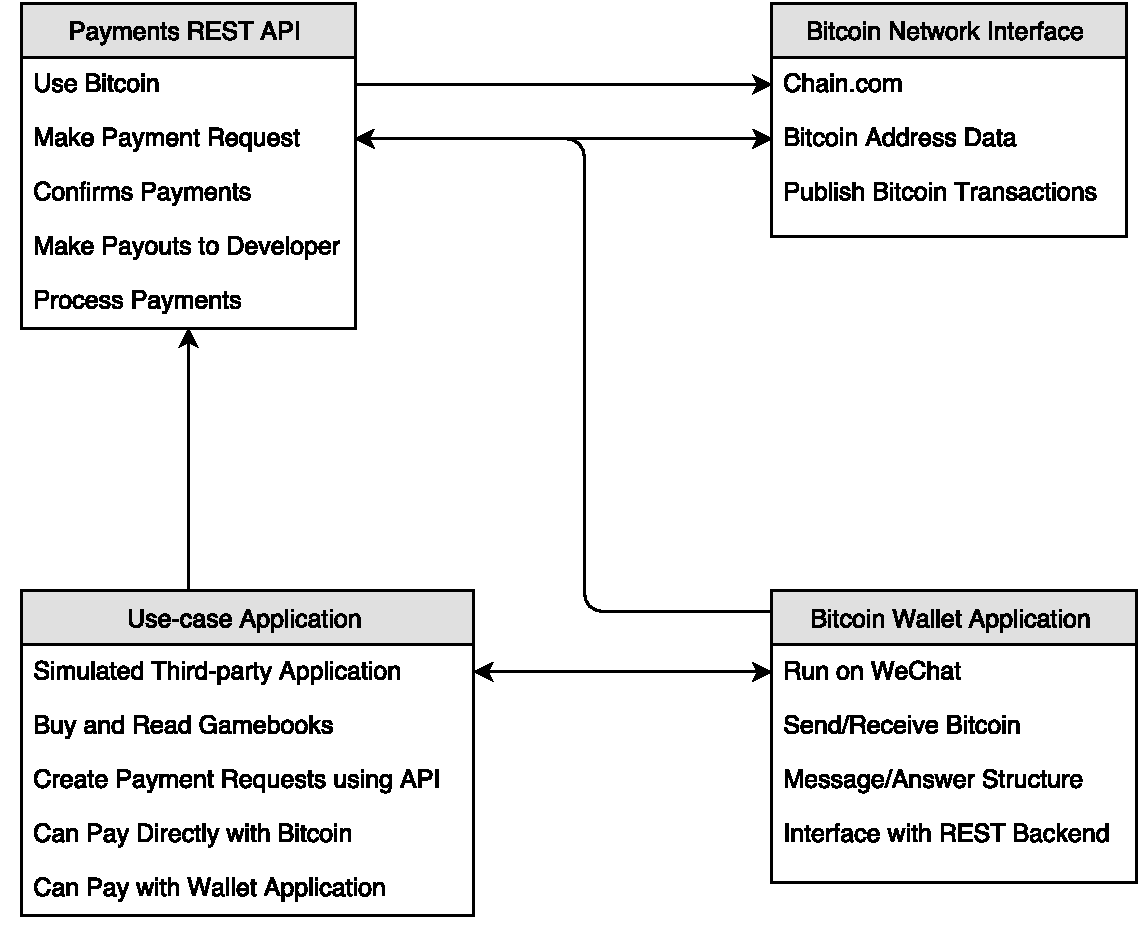
\includegraphics[width=0.7\textwidth]{figs/Summary.pdf}
   \caption{Summary of Framework} 
   \label{fig:summary_framework}
\end{figure}

\subsection{REST API for payment management}

A REST (Representational State Transfer) API \cite{Oracle.com} was chosen for the main interface for developers to use Bitcoin without running a Bitcoin node or having experience with Bitcoin. REST was chosen because it is a commonly used architecture, it is easy to use and understand and it does not constrain the user's choice of programming langauge or environment. 

The purpose of the REST API is to let developers make payment requests and check if a payment has been made, without dealing with the low-level Bitcoin transactions directly. Thus, our system should generate a new Bitcoin address on request. 

% We also require the developer to check wether a payment has been successfully made.
Our requirements from the REST API are:

\begin{itemize}
	\item New Bitcoin address for each payment
	\item Verify payment
	\item Check total balance of developer
	\item Witdraw available Bitcoin of developer
\end{itemize}

\subsubsection{The concept of the Bitcoin payment}

This is a high-level explanation of how to receive verifyable payments with Bitcoin. With Bitcoin, unlike a traditional bank account, you don't have a single ``account'' where people can make payments to and you can verify that the payment came from them. With Bitcoin it is trivially easy to make a new Bitcoin address, and it can be generated without being connected to the Internet or the Bitcoin network.

Since the entire Bitcoin blockchain is public, a single address is not sufficient to receive multiple payments. With a single address, it is not easy to verify that a spesific person has made a payment, since there may be several payments of the same amount happening in short succession.

The sollution to the problem is generating a new address for every payment, and requesting that the user make the payment to that address. Since the newly generated address is not yet present on the blockchain, when a payment to that address of the requested amount occurs, we can be certain that the person in question made the payment. When the payment is complete, the Bitcoin in that address can be transferred to a central address, and the original address can be discarded.

From our requirements for the REST API, we clearly require (at least) the following methods:

\begin{itemize}
	\item A ``payment'' method
	\item A ``balance'' method
	\item A ``payout'' method
\end{itemize}

\subsubsection{The /payment method}
\label{sct:payment}

The /payment method is the core of the REST API. It is used to make a payment request with a specified amount of Bitcoin and a description of the transaction. The /payment method returns a Bitcoin public address and a payment ID. 

The user can then pay to the Bitcoin address using any standard Bitcoin payment method, or can pay directly from the Bitcoin wallet that will run on WeChat and will be connected to the payment infrastructure.

\subsubsection{/payment/\{PUBLIC\_ADDRESS\} and /payment/\{ID\}}

These two methods are conceptually the same, but they take in two different arguments. The one takes the Bitcoin address to be queried, and the other takes the payment ID. The method returns all the data about the transaction, including the status of the transaction. 

The main purpose of this method is to verify that a transaction has been completed by the user. It can also be used to give the payment details to to user again.

\subsubsection{/balance}

The /balance method gives the developer the balance of all the available Bitcoin from all the received transactions. The method also returns a flag that says if there is enough Bitcoin to make a payout.

\subsubsection{/payout}

The /payout method is used by the developer to transfer all of the available Bitcoin to a specified Bitcoin address.

\subsection{Wallet Application}

The Wallet Application is a Bitcoin wallet implemented on the WeChat platform. The WeChat platform uses a simple message-answer structure. A user sends a message in the Wallet Application. The message is then sent to WeChat that sends it to a third party server controlled by the developer. The server then sends a reply to WeChat that is then forwarded to the user. 

In this manner, a fully functional Bitcoin wallet is realised. The third party server stores the private keys and processes the Bitcoin transactions on commands from the user.

The advantage of using the WeChat platform is the security built in to the platform, as well as an existing userbase. 

The Wallet Application will be directly connected to the back-end of the REST API. Thus, payment requests will be referable directly from the Wallet Application without needing to reference the Bitcoin Address. It will be able to reference the request using the payment ID mentioned in \ref{sct:payment}

\subsection{Bitcoin Interface}
\label{sct:bitcoin_interface}

To connect to the Bitcoin peer-to-peer network, a Bitcoin client is needed. The standard way of doing this is running the Bitcoin open source software on a server. This is very network and processor intensive. For development and testing, it will be quite expensive to run the Bitcoin software. Thus, an alternative is required for interfacing with the Bitcoin network. Fortunately, there are services that provide access to most of the Bitcoin operations using their API's. 

We require the following from such a service:

\begin{itemize}
	\item Get the balance from an address,
	\item Get unspent outputs from an address,
	\item Post a signed Bitcoin transaction to the network,
	\item It must be able to use the Testnet
\end{itemize}

The details of the chosen service is covered in chapter \ref{chp:Detail Design}.
% After considering several options, a service called chain.com was chosen. Chain.com is a free service that satisfies all the requirements. It is perfect to use this service as a proof of concept, but in practice one would rather run a full Bitcoin node to minimize reliance on third-party services.

\subsection{Use-case Application}

To use the payment framework, a Gamebook application is created to read Choose Your Own Adventure style books on the WeChat platform. User-created books can be sold by using the Bitcoin payment framework and the author can potentially earn Bitcoin.

For each sale, the Gamebook application creates a payment request using the REST API. The user can then pay using the Wallet Application or any Bitcoin payment mechanism. The Gamebook application can the query the API to confirm that the payment is received. 
%%!TEX root = ../USthesis_Masters.tex
\chapter{System Design}
\label{chp:System Design}


%%%%%%%%%%%%%%%%%%%%%%%%%%%%%%%%%%%%%%%%%%%%%%%%%%%%%%%%%%%%%%%%%%%%%%%
\section{Framework}

In this project we test the viability of a payment framework on a mobile social media platform. The framework will consist of several independant but connected pieces:

\begin{itemize}
	\item REST API for payments
	\item Wallet Application
	\item Bitcoin Interface
	\item Use-case Application
\end{itemize}

A summary of what is required from the system can be seen in figure \ref{fig:summary_framework}.

\begin{figure}
  \centering
    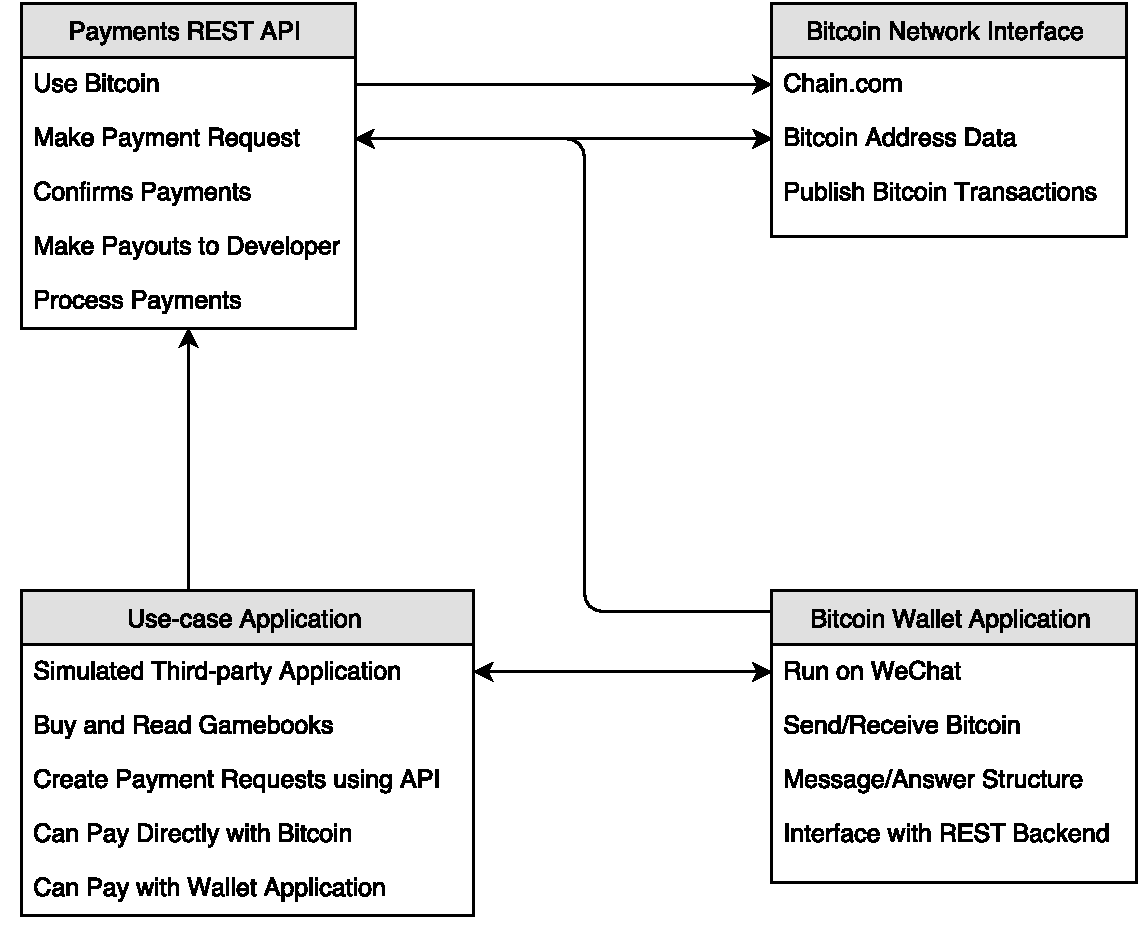
\includegraphics[width=0.7\textwidth]{figs/Summary.pdf}
   \caption{Summary of Framework} 
   \label{fig:summary_framework}
\end{figure}

\subsection{REST API for payment management}

A REST (Representational State Transfer) API \cite{Oracle.com} was chosen for the main interface for developers to use Bitcoin without running a Bitcoin node or having experience with Bitcoin. REST was chosen because it is a commonly used architecture, it is easy to use and understand and it does not constrain the user's choice of programming langauge or environment. 

The purpose of the REST API is to let developers make payment requests and check if a payment has been made, without dealing with the low-level Bitcoin transactions directly. Thus, our system should generate a new Bitcoin address on request. 

% We also require the developer to check wether a payment has been successfully made.
Our requirements from the REST API are:

\begin{itemize}
	\item New Bitcoin address for each payment
	\item Verify payment
	\item Check total balance of developer
	\item Witdraw available Bitcoin of developer
\end{itemize}

\subsubsection{The concept of the Bitcoin payment}

This is a high-level explanation of how to receive verifyable payments with Bitcoin. With Bitcoin, unlike a traditional bank account, you don't have a single ``account'' where people can make payments to and you can verify that the payment came from them. With Bitcoin it is trivially easy to make a new Bitcoin address, and it can be generated without being connected to the Internet or the Bitcoin network.

Since the entire Bitcoin blockchain is public, a single address is not sufficient to receive multiple payments. With a single address, it is not easy to verify that a spesific person has made a payment, since there may be several payments of the same amount happening in short succession.

The sollution to the problem is generating a new address for every payment, and requesting that the user make the payment to that address. Since the newly generated address is not yet present on the blockchain, when a payment to that address of the requested amount occurs, we can be certain that the person in question made the payment. When the payment is complete, the Bitcoin in that address can be transferred to a central address, and the original address can be discarded.

From our requirements for the REST API, we clearly require (at least) the following methods:

\begin{itemize}
	\item A ``payment'' method
	\item A ``balance'' method
	\item A ``payout'' method
\end{itemize}

\subsubsection{The /payment method}
\label{sct:payment}

The /payment method is the core of the REST API. It is used to make a payment request with a specified amount of Bitcoin and a description of the transaction. The /payment method returns a Bitcoin public address and a payment ID. 

The user can then pay to the Bitcoin address using any standard Bitcoin payment method, or can pay directly from the Bitcoin wallet that will run on WeChat and will be connected to the payment infrastructure.

\subsubsection{/payment/\{PUBLIC\_ADDRESS\} and /payment/\{ID\}}

These two methods are conceptually the same, but they take in two different arguments. The one takes the Bitcoin address to be queried, and the other takes the payment ID. The method returns all the data about the transaction, including the status of the transaction. 

The main purpose of this method is to verify that a transaction has been completed by the user. It can also be used to give the payment details to to user again.

\subsubsection{/balance}

The /balance method gives the developer the balance of all the available Bitcoin from all the received transactions. The method also returns a flag that says if there is enough Bitcoin to make a payout.

\subsubsection{/payout}

The /payout method is used by the developer to transfer all of the available Bitcoin to a specified Bitcoin address.

\subsection{Wallet Application}

The Wallet Application is a Bitcoin wallet implemented on the WeChat platform. The WeChat platform uses a simple message-answer structure. A user sends a message in the Wallet Application. The message is then sent to WeChat that sends it to a third party server controlled by the developer. The server then sends a reply to WeChat that is then forwarded to the user. 

In this manner, a fully functional Bitcoin wallet is realised. The third party server stores the private keys and processes the Bitcoin transactions on commands from the user.

The advantage of using the WeChat platform is the security built in to the platform, as well as an existing userbase. 

The Wallet Application will be directly connected to the back-end of the REST API. Thus, payment requests will be referable directly from the Wallet Application without needing to reference the Bitcoin Address. It will be able to reference the request using the payment ID mentioned in \ref{sct:payment}

\subsection{Bitcoin Interface}
\label{sct:bitcoin_interface}

To connect to the Bitcoin peer-to-peer network, a Bitcoin client is needed. The standard way of doing this is running the Bitcoin open source software on a server. This is very network and processor intensive. For development and testing, it will be quite expensive to run the Bitcoin software. Thus, an alternative is required for interfacing with the Bitcoin network. Fortunately, there are services that provide access to most of the Bitcoin operations using their API's. 

We require the following from such a service:

\begin{itemize}
	\item Get the balance from an address,
	\item Get unspent outputs from an address,
	\item Post a signed Bitcoin transaction to the network,
	\item It must be able to use the Testnet
\end{itemize}

The details of the chosen service is covered in chapter \ref{chp:Detail Design}.
% After considering several options, a service called chain.com was chosen. Chain.com is a free service that satisfies all the requirements. It is perfect to use this service as a proof of concept, but in practice one would rather run a full Bitcoin node to minimize reliance on third-party services.

\subsection{Use-case Application}

To use the payment framework, a Gamebook application is created to read Choose Your Own Adventure style books on the WeChat platform. User-created books can be sold by using the Bitcoin payment framework and the author can potentially earn Bitcoin.

For each sale, the Gamebook application creates a payment request using the REST API. The user can then pay using the Wallet Application or any Bitcoin payment mechanism. The Gamebook application can the query the API to confirm that the payment is received. 

%==== Appendices ====================================================
\appendix
\appendixpage\relax

\chapter{No appendices yet}
% \label{chp:DEM-Theory}

% \section{Ball elements}
% \label{sec:Ball-elems}

% \begin{figure}
%    \centering
%    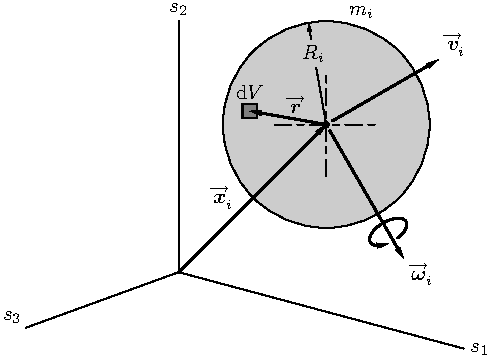
\includegraphics{figs/DEM-Def-Ball}
%    \caption{Ball Element Parameters}
%    \label{fig:BallDef}
% \end{figure}


% \subsection{Ball mass and inertia parameters}

% Consider a volume element $\mathrm{d}V$ with respect to a static base $S$ of
% an arbitrary solid body with  density $\rho$. The mass of the body is
% obtained by integrating over the volume of the body,
% \begin{equation}
%     m = \int\limits_{\mathrm{body}} \rho\, \mathrm{d}V
%     \label{eq:BMass-dif}
% \end{equation}

% In figure~\ref{fig:BallDef}, a ball with radius $R_{i}$ and uniform density
% $\rho_i$ is depicted. The mass of the ball is after integration of
% equation~\eqref{eq:BMass-dif}
% \begin{equation}
%     m_i = \tfrac{4}{3} \pi \rho_i\, R_i^3 .
%     \label{eq:BMass}
% \end{equation}


%----------------------------------------------------------------------------
\endinput

%\include{contents/App-2}
%\include{contents/App-3}

%==== Bibliography acro's & Index ===================================
\backmatter

\bibliography{backmatter/Thesis}

\end{document}
